\documentclass{beamer}


\usepackage{amsmath}
\usepackage{bookmark}
\usepackage{graphicx}
\usepackage{tikz-cd}
\usepackage{quiver}
\usepackage{mathtools}
\usepackage{bbm}


\usetheme{metropolis}

\mode<presentation>

%Information to be included in the title page:
\title{Modeling Complex Systems \\with Category Theory}
\author{Daniel Sinderson}
\institute{Southern Oregon University}
\date{2024}

\begin{document}

\frame{\titlepage}

%\begin{frame}
%    \frametitle{Table of Contents}
%    \tableofcontents
%\end{frame}


%%%%%%%%%%%%%%%%%%%%%%%%%%%%%%%%%%%%%%%%%%%%%%%%%%%%%%%%%%%%%%%%%%%%%%%%%%%%%%%%%%%%%%%%%%%
%%%%%%%%%%%%%%%%%%%%%%%%%%%%%%%%%%%%%%%%%%%%%%%%%%%%%%%%%%%%%%%%%%%%%%%%%%%%%%%%%%%%%%%%%%%
\section{Objective and Scope of the Project}
%%%%%%%%%%%%%%%%%%%%%%%%%%%%%%%%%%%%%%%%%%%%%%%%%%%%%%%%%%%%%%%%%%%%%%%%%%%%%%%%%%%%%%%%%%%
%%%%%%%%%%%%%%%%%%%%%%%%%%%%%%%%%%%%%%%%%%%%%%%%%%%%%%%%%%%%%%%%%%%%%%%%%%%%%%%%%%%%%%%%%%%

\begin{frame}
    \frametitle{Scope of the Project}
    My objective for this project was to learn about the brand new field of categorical systems theory
    , which applies the pure math field of category theory to the study of arbitrary systems
    , and then use the tools that I learned to model a complex real-world system.

    \vspace*{0.25in}

    But I didn't know category theory or any complex systems...
\end{frame}

\begin{frame}
    \frametitle{The Actual Scope of the Project}
    \begin{enumerate}
        \item Learn Category Theory
        \item Learn Categorical Systems Theory
        \item Learn about a real world system (Transcription Networks)
        \item Learn how to use the AlgebraicDynamics library written in the Julia programming language
        \item Model it and simulate the results
        \item Live to tell you all about it
    \end{enumerate}
\end{frame}

\begin{frame}
    \frametitle{Scope of this Presentation}
    Keep things high-level and descriptive and move fast.

    \vspace*{0.125in}

    \begin{enumerate}
        \item Tell you what a system is.
        \item Tell you what a category is.
        \item Tell you how they can work together.
        \item Show you a complex system and how I modeled it.
        \item Talk about the simulation results.
    \end{enumerate}
\end{frame}



%%%%%%%%%%%%%%%%%%%%%%%%%%%%%%%%%%%%%%%%%%%%%%%%%%%%%%%%%%%%%%%%%%%%%%%%%%%%%%%%%%%%%%%%%%%
%%%%%%%%%%%%%%%%%%%%%%%%%%%%%%%%%%%%%%%%%%%%%%%%%%%%%%%%%%%%%%%%%%%%%%%%%%%%%%%%%%%%%%%%%%%
\section{Systems}
%%%%%%%%%%%%%%%%%%%%%%%%%%%%%%%%%%%%%%%%%%%%%%%%%%%%%%%%%%%%%%%%%%%%%%%%%%%%%%%%%%%%%%%%%%%
%%%%%%%%%%%%%%%%%%%%%%%%%%%%%%%%%%%%%%%%%%%%%%%%%%%%%%%%%%%%%%%%%%%%%%%%%%%%%%%%%%%%%%%%%%%


\begin{frame}{What is a System?}
    A system is a thing that changes. At it's simplest, a system consists of the following two things.

    \begin{enumerate}
        \item A set of states that the system can be in.
        \item A map that updates the system's state based on the state that it's currently in.
    \end{enumerate}

    \begin{center}
        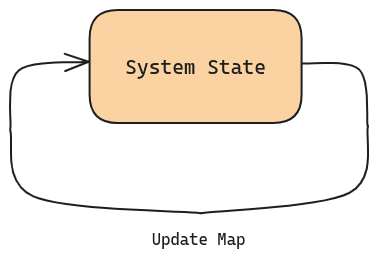
\includegraphics[scale=0.35]{system_diagram_closed.png}
    \end{center}

\end{frame}


\begin{frame}{Examples of Systems}
    The set of natural numbers with the successor function is a system.
    \vspace*{0.125in}
    \[
        S: \mathbb{N} \rightarrow \mathbb{N}
    \]
    \[
        \ \ \ \ \ \ \ \ \ n \mapsto n+1
    \]
\end{frame}


\begin{frame}{Examples of Systems}
    An ordinary differential equation is also a system.
    \vspace*{0.125in}
    \[
        \frac{dx}{dt}=\kappa x
    \]
    Here the set of states is the set of real numbers $\mathbb{R}$ and the update map is the differential equation itself: given the current state, $x$, the differential equation tells us how to change it.
\end{frame}


\begin{frame}{What's the Problem}
    The problem with these systems is that they're closed.

    \vspace*{0.125in}
    They don't interact with each other. And they don't interact with their environment.

    \vspace*{0.125in}
    So let's open them up with category theory.
\end{frame}







%%%%%%%%%%%%%%%%%%%%%%%%%%%%%%%%%%%%%%%%%%%%%%%%%%%%%%%%%%%%%%%%%%%%%%%%%%%%%%%%%%%%%%%%%%%
%%%%%%%%%%%%%%%%%%%%%%%%%%%%%%%%%%%%%%%%%%%%%%%%%%%%%%%%%%%%%%%%%%%%%%%%%%%%%%%%%%%%%%%%%%%
\section{Categories}
%%%%%%%%%%%%%%%%%%%%%%%%%%%%%%%%%%%%%%%%%%%%%%%%%%%%%%%%%%%%%%%%%%%%%%%%%%%%%%%%%%%%%%%%%%%
%%%%%%%%%%%%%%%%%%%%%%%%%%%%%%%%%%%%%%%%%%%%%%%%%%%%%%%%%%%%%%%%%%%%%%%%%%%%%%%%%%%%%%%%%%%

\begin{frame}{Category Theory Basics}
    Category theory is a theory of structure and composition.

    \vspace*{0.25in}
    It uses the mathematical object of a category to encapsulate the notion of associative composition.

    \vspace*{0.25in}
    With this alone it creates a language capable of formalizing all of mathematics.
\end{frame}


\begin{frame}{What is a Category?}
    \begin{definition}[Category]
        A category $\mathcal{C}$ is defined by the following:
        \begin{enumerate}
            \item $\mathcal{C}$ contains a collection of objects $\mathsf{ob}(\mathcal{C})$.
            \item For any two objects $a$, $b$ $\in \mathcal{C}$ there is a collection of morphisms, $f:a \rightarrow b$, between those objects called the homset, $\mathcal{C}(a,b)$ .
            \item Every object $a\in \mathcal{C}$ has a morphism to itself $\mathsf{id}_a:a\rightarrow a$ called its identity.
            \item For every two morphisms $f:a\rightarrow b$ and $g: b\rightarrow c$ there's a third morphism $g\circ f:a\rightarrow c$ that's their composition.
        \end{enumerate}
    \end{definition}
\end{frame}


\begin{frame}[fragile]{What is a Category?}
    These objects and morphisms are then under two constraints: unitality and associativity.
    \begin{definition}[Category cont. Unitality]
        Any morphism $f:a\rightarrow b$ can be composed with the identity morphisms of $a$ and $b$ such that $f\circ \mathsf{id}_a=\mathsf{id}_b\circ f=f$.
        \[\begin{tikzcd}
                a && b \\
                \\
                a && b
                \arrow["f", from=1-1, to=1-3]
                \arrow["{\mathsf{id}_a}"', from=1-1, to=3-1]
                \arrow["{\mathsf{id}_b}", from=1-3, to=3-3]
                \arrow["f"', from=3-1, to=3-3]
            \end{tikzcd}\]
    \end{definition}
\end{frame}


\begin{frame}[fragile]{What is a Category?}
    These objects and morphisms are then under two constraints: unitality and associativity.
    \begin{definition}[Category cont. Associativity]
        For any morphisms $f:a\rightarrow b$, $g:b\rightarrow c$, and $h:c\rightarrow d$, $h\circ (g\circ f)=(h\circ g)\circ f$. Since it doesn't matter what order we apply the morphisms, we write this $h\circ g \circ f$.
        \[\begin{tikzcd}
                a & b & c & d
                \arrow["f"', from=1-1, to=1-2]
                \arrow["g"', from=1-2, to=1-3]
                \arrow["h"', from=1-3, to=1-4]
                \arrow["{{g\circ f}}", curve={height=-24pt}, from=1-1, to=1-3]
                \arrow["{{h\circ g}}"', curve={height=24pt}, from=1-2, to=1-4]
            \end{tikzcd}\]
    \end{definition}
\end{frame}

%\begin{frame}{Monoidal Categories}
%    To build systems compositionally we'll also need a way to place them in parallel.
%
%    \vspace*{0.125in}
%    Similar to a binary operation on a set, we can have a binary operation on a category.
%
%    \vspace*{0.125in}
%    This construction is captured in the notion of a monoidal category.
%\end{frame}
%
%
%\begin{frame}{Monoidal Categories}
%    \begin{definition}[Monoidal Categories]
%        A category $\mathcal{C}$ is monoidal if the following exist.
%        \begin{enumerate}
%            \item A functor $\otimes:\mathcal{C}\times\mathcal{C}\rightarrow\mathcal{C}$ called the monoidal product.
%            \item An object $\mathbbm{1}\in\mathcal{C}$ called the unit.
%            \item A natural isomorphism $\alpha : (a\otimes b)\otimes c\Rightarrow a\otimes (b\otimes c)$ called the associator, with components $\alpha_{x,y,z}: (x\otimes y)\otimes z\rightarrow x\otimes (y\otimes z)$.
%            \item A natural isomorphism $\lambda : \mathbbm{1}\otimes a\Rightarrow a$ called the left unitor with components $\lambda_x : \mathbbm{1}\otimes x\rightarrow x$.
%            \item A natural isomorphism $\rho : a\otimes \mathbbm{1}\Rightarrow a$ called the right unitor with components $\lambda_x : x\otimes \mathbbm{1}\rightarrow x$.
%        \end{enumerate}
%    \end{definition}
%\end{frame}
%
%\begin{frame}[fragile]{Monoidal Categories}
%    \begin{definition}[Monoidal Categories]
%        All of the above must exist such that the following two diagrams, called the triangle identity and the pentagon identity, commute.
%
%        \vspace*{0.5in}
%        \[\begin{tikzcd}
%                {(x\otimes\mathbbm{1})\otimes y} && {x\otimes(\mathbbm{1}\otimes y)} \\
%                \\
%                && {x\otimes y}
%                \arrow["{{\rho_x\otimes \mathsf{id}_y}}"', from=1-1, to=3-3]
%                \arrow["{{\mathsf{id}_x\otimes\lambda_y}}", from=1-3, to=3-3]
%                \arrow["{{\alpha_{x,y,z}}}", from=1-1, to=1-3]
%            \end{tikzcd}\]
%    \end{definition}
%\end{frame}
%
%\begin{frame}[fragile]{Monoidal Categories}
%    \begin{definition}[Monoidal Categories]
%        All of the above must exist such that the following two diagrams, called the triangle identity and the pentagon identity, commute.
%
%        \vspace*{0.125in}
%        \[\begin{tikzcd}
%                {((w\otimes x)\otimes y)\otimes z} && {(w\otimes x)\otimes(y\otimes z)} \\
%                \\
%                {(w\otimes (x\otimes y))\otimes z} \\
%                \\
%                {w\otimes ((x\otimes y)\otimes z)} && {w\otimes (x\otimes (y\otimes z))}
%                \arrow["{{\alpha_{w,x,(y\otimes z)}}}", from=1-3, to=5-3]
%                \arrow["{{\alpha_{(w\otimes x),y,z}}}", from=1-1, to=1-3]
%                \arrow["{{\alpha_{w,x,y}\otimes \mathsf{id}_z}}"', from=1-1, to=3-1]
%                \arrow["{{\alpha_{w,(x\otimes y),z}}}"', from=3-1, to=5-1]
%                \arrow["{{\mathsf{id}_w\otimes \alpha_{x,y,z}}}"', from=5-1, to=5-3]
%            \end{tikzcd}\]
%    \end{definition}
%\end{frame}
%
%%%%%%%%%%%%%%%%%%%%%%%%%%%%%%%%%%%%%%%%%%%%%%%%%%%%%%%%%%%%%%%%%%%%%%%%%%%%%%%%%%%%%%%%%%%%
%%%%%%%%%%%%%%%%%%%%%%%%%%%%%%%%%%%%%%%%%%%%%%%%%%%%%%%%%%%%%%%%%%%%%%%%%%%%%%%%%%%%%%%%%%%
\section{Composing Systems}
%%%%%%%%%%%%%%%%%%%%%%%%%%%%%%%%%%%%%%%%%%%%%%%%%%%%%%%%%%%%%%%%%%%%%%%%%%%%%%%%%%%%%%%%%%%
%%%%%%%%%%%%%%%%%%%%%%%%%%%%%%%%%%%%%%%%%%%%%%%%%%%%%%%%%%%%%%%%%%%%%%%%%%%%%%%%%%%%%%%%%%%
\begin{frame}{What is a Open System?}
    An open system is as a system with an interface.

    \vspace*{0.125in}
    \begin{center}
        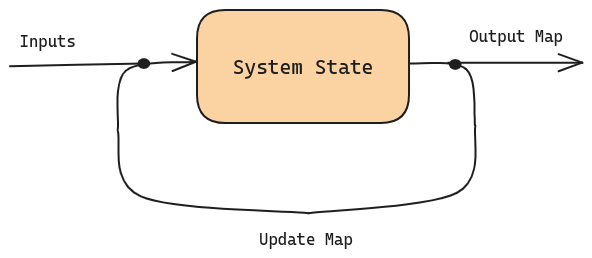
\includegraphics[scale=0.35]{system_diagram_open.png}
    \end{center}
\end{frame}


\begin{frame}{Lenses and Arenas}
    To model this mathematically we'll use objects called arenas and morphisms called lenses.

    \vspace*{0.125in}
    \begin{definition}[Arenas]
        An arena is a pair of objects $\begin{pmatrix}A \\ B\end{pmatrix}$ from an underlying category.
    \end{definition}

    \begin{definition}
        A lens is a morphism between arenas made from a pair of morphisms from the underlying category
        $$\begin{pmatrix}f \\ g\end{pmatrix}: \begin{pmatrix}A \\ B\end{pmatrix} \leftrightarrows \begin{pmatrix}C \\ D\end{pmatrix}$$
        where $f:B\rightarrow D$ is the output map and $g:B\times C \rightarrow A$ is the update map.
    \end{definition}
\end{frame}


\begin{frame}{What this Gives Us}
    Arenas and lenses between them form a monoidal category.

    \vspace*{0.125in}
    This means that we can compose systems and multiply them.

    \vspace*{0.125in}
    By modeling our open systems as lenses, composition of lenses lets us place systems in series and multiplication of lenses lets us place systems in parallel.
\end{frame}


\begin{frame}{Systems in Series and Parallel}
    \begin{center}
        Systems in Series:
        $\begin{pmatrix}g^\# \\ g\end{pmatrix} \circ \begin{pmatrix}f^\# \\ f\end{pmatrix}$

        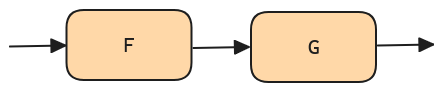
\includegraphics[scale=0.25]{Systems_Series.png}

        \vspace*{0.25in}
        Systems in Parallel:
        $\begin{pmatrix}g^\# \\ g\end{pmatrix} \otimes \begin{pmatrix}f^\# \\ f\end{pmatrix}$

        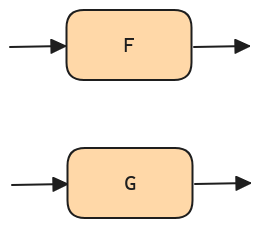
\includegraphics[scale=0.25]{Systems_Parallel.png}

    \end{center}




\end{frame}

%%%%%%%%%%%%%%%%%%%%%%%%%%%%%%%%%%%%%%%%%%%%%%%%%%%%%%%%%%%%%%%%%%%%%%%%%%%%%%%%%%%%%%%%%%%
%%%%%%%%%%%%%%%%%%%%%%%%%%%%%%%%%%%%%%%%%%%%%%%%%%%%%%%%%%%%%%%%%%%%%%%%%%%%%%%%%%%%%%%%%%%
\section{Case Study}
%%%%%%%%%%%%%%%%%%%%%%%%%%%%%%%%%%%%%%%%%%%%%%%%%%%%%%%%%%%%%%%%%%%%%%%%%%%%%%%%%%%%%%%%%%%
%%%%%%%%%%%%%%%%%%%%%%%%%%%%%%%%%%%%%%%%%%%%%%%%%%%%%%%%%%%%%%%%%%%%%%%%%%%%%%%%%%%%%%%%%%%

\begin{frame}{Gene Transcription}
    Gene transcription is the process by which genes in a cell’s DNA produce proteins.

    \vspace*{0.125in}
    The dynamics of this process for a single gene are well modeled by the following differential equation, where $f(X^*)$ is the activation function of the gene.
    $$\frac{dY}{dt}=\beta f(X^*) - \alpha Y$$

    $$\text{Activator: } \ f(X^*)=\frac{\beta X^{*n}}{K^n + X^{*n}} \ \text{ or } \ \beta * P(X^* > K)$$
    $$\text{Repressor: } \ f(X^*)=\frac{\beta}{1 + \left(\frac{X^*}{K}\right)^n} \ \text{ or } \ \beta * P(X^* < K)$$
\end{frame}

\begin{frame}{Motor Flagella Network}
    Gene transcription network are connected networks of genes whose products act as transcription factors for other genes.

    \vspace*{0.125in}
    Below is the motor flagella network of \textit{e. coli} bacteria.

    \begin{center}
        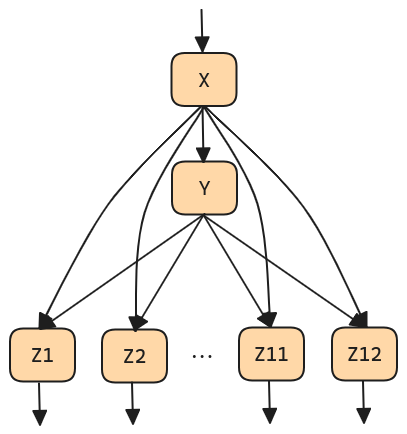
\includegraphics[scale=0.25]{multioutput_FFL_color.png}
        \hspace*{0.25in}
        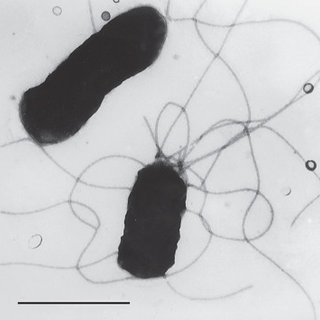
\includegraphics[scale=0.35]{Flagella-of-E-coli-observed-in-transmission-electron-microscope-Bar-1mm_Q320-2724765803.jpg}
    \end{center}

    \begin{footnotesize}
        \hspace*{\fill}Image from \textit{Bacterial Chemotaxis} by Michael Eisenbach
    \end{footnotesize}
\end{frame}


\begin{frame}{Motor Flagella Network Model}
    Using lenses we can wire together the transcription factor dynamics as differential systems and then simulate the results.

    \begin{center}
        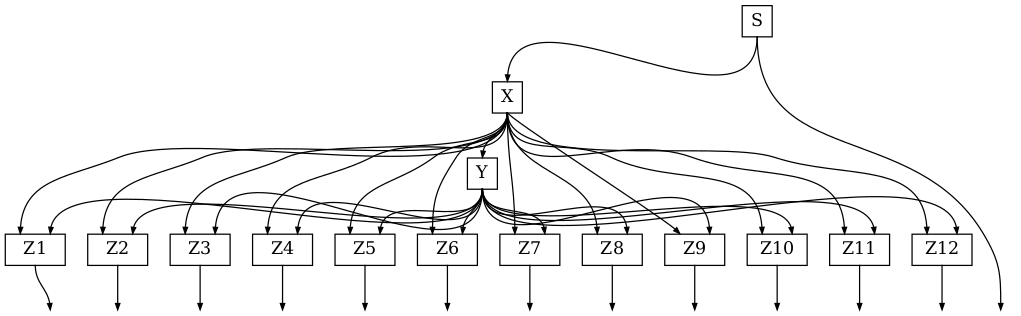
\includegraphics[scale=0.35]{motor_flagella_network.png}
    \end{center}

\end{frame}

\begin{frame}{Motor Flagella Network Simulation Results}

    \begin{center}
        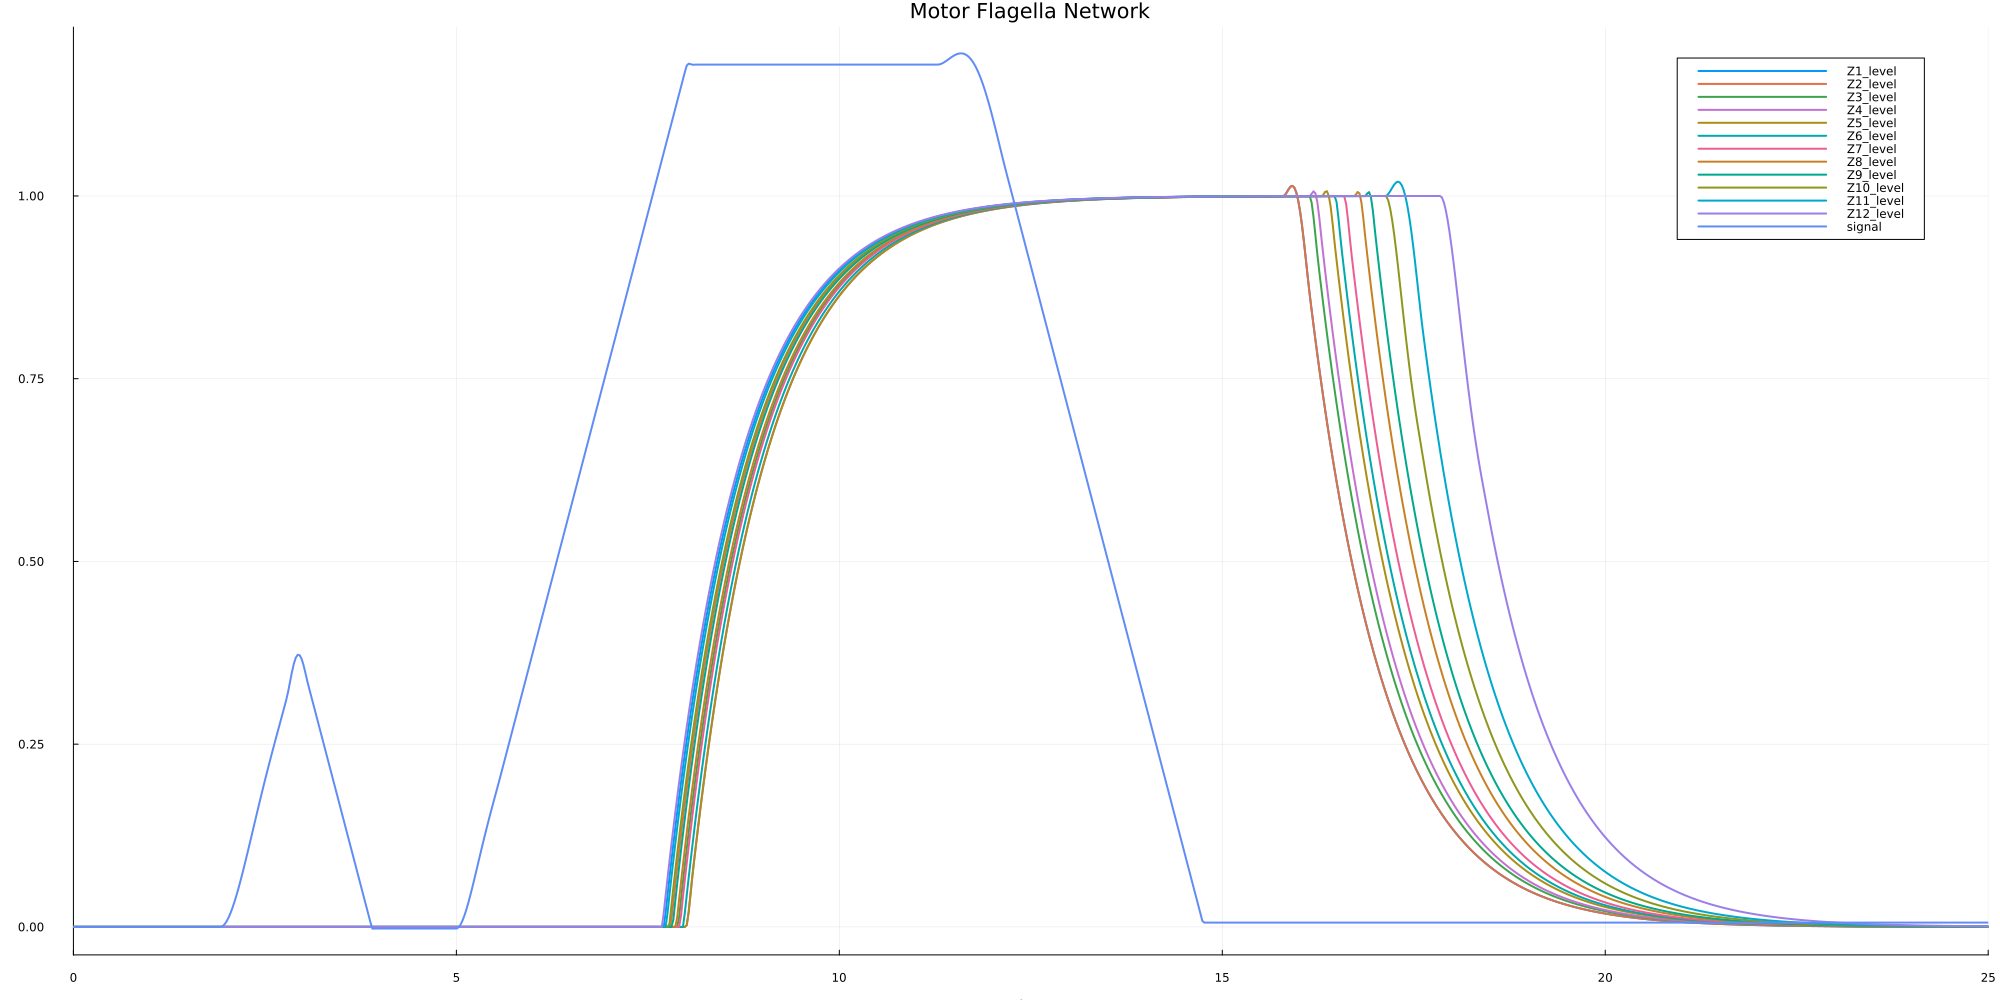
\includegraphics[scale=0.20]{motor_flagella.png}
    \end{center}
\end{frame}


%%%%%%%%%%%%%%%%%%%%%%%%%%%%%%%%%%%%%%%%%%%%%%%%%%%%%%%%%%%%%%%%%%%%%%%%%%%%%%%%%%%%%%%%%%%
%%%%%%%%%%%%%%%%%%%%%%%%%%%%%%%%%%%%%%%%%%%%%%%%%%%%%%%%%%%%%%%%%%%%%%%%%%%%%%%%%%%%%%%%%%%
\section{Conclusion}
%%%%%%%%%%%%%%%%%%%%%%%%%%%%%%%%%%%%%%%%%%%%%%%%%%%%%%%%%%%%%%%%%%%%%%%%%%%%%%%%%%%%%%%%%%%
%%%%%%%%%%%%%%%%%%%%%%%%%%%%%%%%%%%%%%%%%%%%%%%%%%%%%%%%%%%%%%%%%%%%%%%%%%%%%%%%%%%%%%%%%%%


\begin{frame}{Where did all the Category Theory Go?}

    It's inside the visual formalism of the wiring diagrams.

    \vspace*{0.5in}
    Diagrammatic languages are more intellectually tractable.

    \vspace*{0.5in}
    They are easier to reason about for both the designer or modeler and those they are designing or modeling for.

\end{frame}


\begin{frame}{What's Next?}
    Lenses over other cartesian categories: $\textbf{Set}$, $\textbf{Man}$

    \vspace*{0.5in}
    Adding monads for nondeterministic systems: MDP, SDE

    \vspace*{0.5in}
    Using charts and double categories to compose system behavior as well as specification
\end{frame}




\begin{frame}{}
    \begin{center}
        \begin{Huge}
            Thank You!
        \end{Huge}
    \end{center}
\end{frame}


\begin{frame}{References}
    \begin{thebibliography}{10}

        \bibitem{alon2019introduction}
        {\sc Alon, U.}
        \newblock {\em An introduction to systems biology: design principles of biological circuits}.
        \newblock Chapman and Hall/CRC, 2019.

        \bibitem{fong2019invitation}
        {\sc Fong, B., and Spivak, D.~I.}
        \newblock {\em An invitation to applied category theory: seven sketches in compositionality}.
        \newblock Cambridge University Press, 2019.

        \bibitem{myers2022categorical}
        {\sc Myers, D.~J.}
        \newblock Categorical systems theory.
        \newblock {\em Manuscript in preparation\/} (2022).
    \end{thebibliography}
\end{frame}



\end{document}